%!TEX root = main.tex

\section{Introduction}

\noindent A key challenge facing Internet services today is how to share resources across users to maximize the user-perceived {\em QoE} (Quality of Experience) by minimizing their end-to-end delay.
Maintaining desirable level of user-perceived QoE is critical, with reducing a few hundred milliseconds from the page load time means millions of dollars.
%The fundamental challenge facing large-scale web service providers and (\eg Microsoft, Facebook, Akamai, Google, Amazon) is how the backend systems should share its resources in order to optimize user-perceived {\em QoE} (Quality of Experience). 
%Maintaining desirable level of user-perceived QoE critical for their revenue models.
A delay penalty of 400ms in Google search responses reduces search volume by 0.74\%; and 500ms of latency for Bing decreases revenue by 1.2\%~\cite{google-revenue,bing-revenue}; For Amazon, an additional latency of 100ms means a 1\% drop in sales~\cite{amazon-revenue}.
Yet, despite substantial efforts (\eg~\cite{shandian,gaze,rosen2017push,jalaparti2013speeding}), maintaining desirable QoE remains a challenge, with average page loading time of Facebook requests being over 3000ms~\cite{mystery}.
% with 50\% users of some popular website spending over 30\% of page loading time on the web backend~\cite{mystery}.

We argue that the key missing piece of today's Internet architecture is that individual Internet systems, \eg web backends, CDNs, and ISPs, are agnostic to their impact on individual users' real-time QoE, especially the difference in their impact across users.
As a consequence, it is difficult for these systems to direct optimizes QoE. 
Instead, our overarching thesis that these systems should be driven directly by the real-time information about their impact on the QoE across users, which could substantially improve QoE as well as resource efficiency, without adding new resources.
While there have been similar efforts in the past (\eg~\cite{alto,frank2013pushing,xie2008p4p,jiang2009cooperative}) toward similar end-to-end quality optimization, our project is inspired by several favorable recent trends, including ``use-case pulls'', \eg the prevalence of QoE-driven revenue models (\eg~\cite{akamai-report,dobrian2011understanding}), as well as ``technological pushes'', \eg the wide use of tracing from the clients and the backend systems (\eg~\cite{mystery,zhao2014lprof}). 

This proposal explores the benefits and challenges of our thesis in the context of how web backend systems should optimize web QoE by leveraging user heterogeneity. 

\mypara{Limitation of today's web backend}
%The web backend systems today have no direct visibility of the QoE of each web request when it arrives, 
Because the end-to-end delay (page loading time) of a web request is affected by the delay of many non-backend systems (ISPs, client-side software, etc) which is beyond the scope of the web service providers, the web backend systems have no direct visibility of how much impact it has on the QoE of individual requests.
As a result, the web backend systems seek to minimize the overall {\em backend delay} (\eg the mean, tail values, or the probability of missing some SLA deadline), under the assumption that backend delay of $n$~ms has the {\em same} impact on any request.\footnote{Modulo the content-specific (\eg web page type) or user-specific (\eg free vs. premium subscription) factors.}
%Page load time, which we refer to as {\em end-to-end delay}, generally consists of three parts: client-side delay, wide-area network (WANs) delay, and backend delay.
%- Web services, like applications running in the cloud, have been basing their optimizations on the goal of improving server-side latency (sometimes the fraction of users meeting some fixed deadline)
%Because of the federated nature of Internet architecture, web service providers do not have full control over all types of delays.
%---to them, WANs and clients devices are largely blackboxes operated, not by the web services, but by ISPs, cellular carriers, and device vendors.
%(while web browsers and apps are developed by the web service providers, the client-side performance is largely decided by how OS share resources among multiple applications).
%With web service providers only controlling the web backend, the performance metric they focus on optimizing is the 
%%Thus, instead of optimizing for QoE directly, today's web services focus on reducing the 
%%different requests have the same {\em QoE sensitivity to backend delay}
%{\em backend delay}, under the assumption that a backend delay of $n$~ms has the {\em same} impact on any request.\footnote{Modulo the content-specific (\eg web page type) or user-specific (\eg free vs. premium subscription) factors.}
% That is, a backend delay of $n$~ms has the same effect on the QoE of any request.
%For instance, they minimize the mean/tail backend delay or the fraction of requests whose backend delay exceeds some deadline (\eg 300ms)~\cite{??,??}.
%- This project takes a step back and asks a different question: does the latency have the same impact on user QoE? 
% In doing so, 
%all requests are optimized with the same objective function of backend response time; 
% an implicit assumption is that different requests have the same {\em QoE sensitivity to backend delay} (modulo content-/user-specific factors, such as web page type or subscription type, etc);
% that is, a backend delay of $n$~ms has the same effect on the QoE of different requests.

We take a step back, and ask {\em ``does the backend delay really have the same impact the QoE of any web request?''}
%- The answer is no, which has profound impact on how web services should be built. [Give a simple example here.] In essence, this means giving each ``priority'', in terms of resources and scheduling, is cost-inefficient and suboptimal. [Give a simple example. resources wasted for users who are screwed already]
Our answer is {\em no}, and such heterogeneous sensitivity of QoE to backend delay is pervasive among requests of the same application. 
This is due to the fact that how much impact the backend delay has on a request depends on the non-backend delay experienced by a request (\eg ISP routing, client-side resource allocation by the device OS), which can have a great variability among requests and over time~\cite{timecard,dqbarge}.
%Two observations contribute to this conclusion: the non-linear relationship between page load time and QoE~\cite{??} and the fact that the WAN/client delay varies among requests~\cite{timecard,dqbarge}, {\em the QoE sensitivity to backend delay varies among requests.}
For instance, the QoE of a web request that has spent 50ms on wide-area networks tends to be more sensitive to 10ms backend delay than a request that has already spent 500ms on the network.
By falsely assuming requests are equally sensitive to the backend delay, traditional web backend system (Figure~\ref{fig:intro-overview}(a)) might waste resources on requests that are insensitive to the backend delay, and/or have suboptimal QoE (\eg using inadequate resources on requests whose QoE is critically dependent on the backend delay. 

\mypara{Our approach} 
This proposal introduces ``QoE sensitivity'' as a new dimension for web QoE optimization, and propose to develop {\bf QoE-driven web backend} systems (Figure~\ref{fig:intro-overview}(b)). 
We argue that embracing the heterogeneity in QoE's sensitivity to backend delay has profound implications for backend systems: 
it should allocate resources in a way that favors the requests whose QoE is more sensitive to backend delay to improve the overall QoE while having minimal drop in the QoE of other requests.
For instance, in a trace-driven simulation (\S\ref{sec:quantifying}), we found that a simple QoE-driven resource allocation policy can raise user experience (measured in user engagement) 50\% closer to optimal (\ie zero backend delay) than a QoE-agnostic baseline web backend.
%should allocate their limited resources. 
%By taking into account the QoE's sensitivity to the backend delay, 
%\jc{bring up some concrete improvement numbers}
%\jc{need to highlight that this is not because application differents}

\begin{figure}[t]
	\centering
	\vspace{-0.5cm}
%	\hspace{0.6cm}
	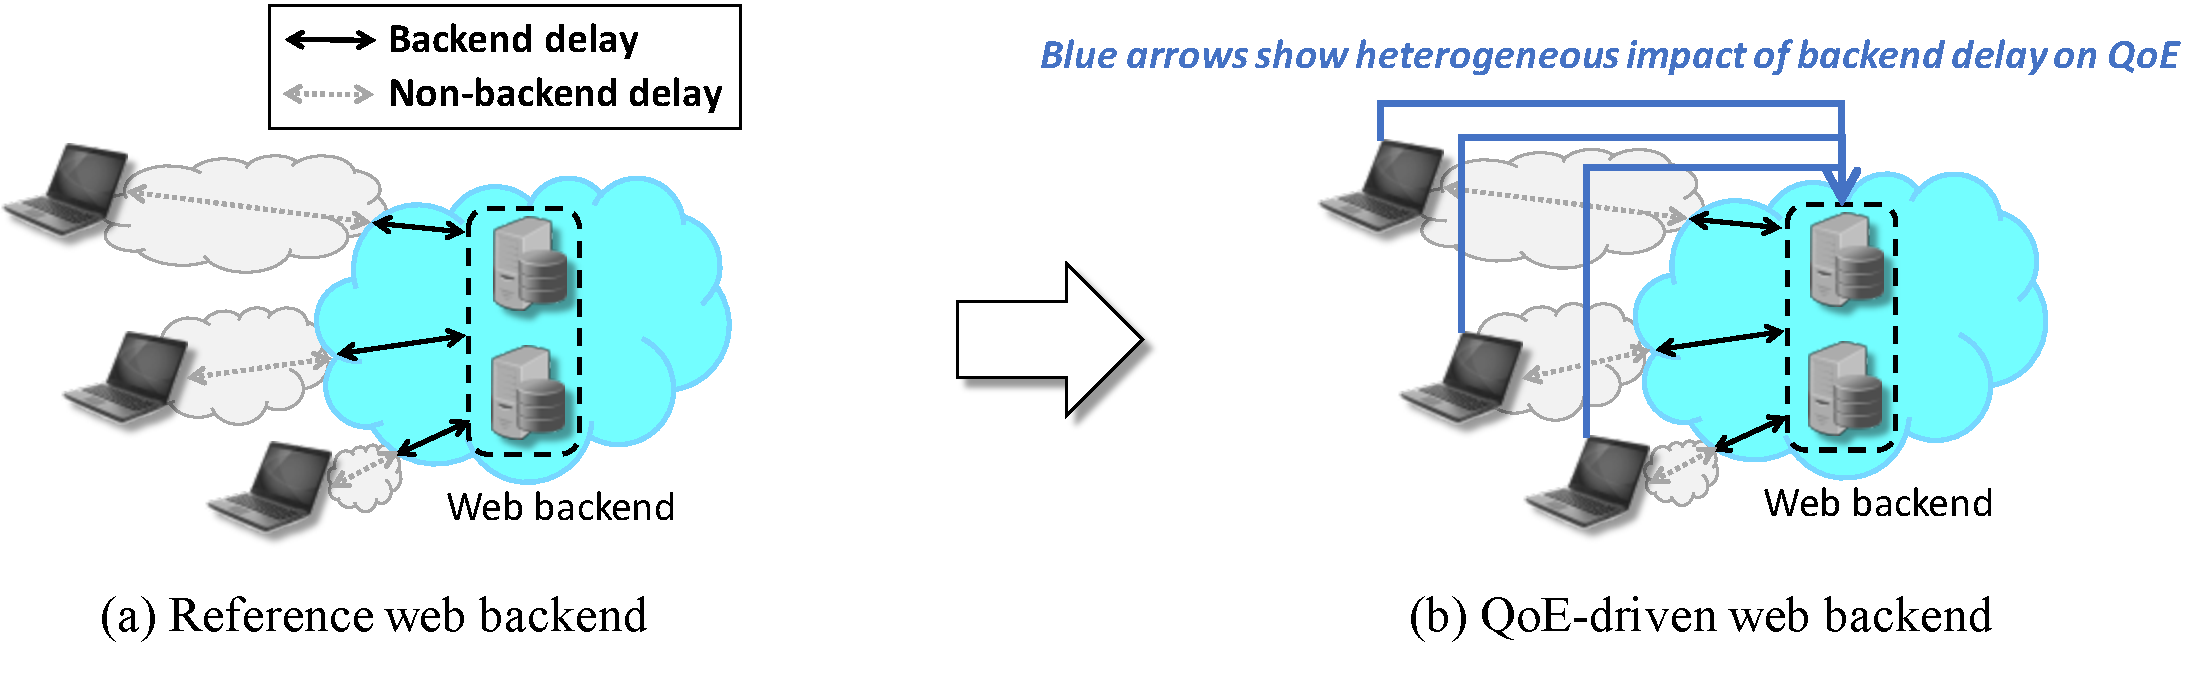
\includegraphics[width=0.75\textwidth]{figs/intro-overview-new.pdf}
	\vspace{-0.1cm}
	\tightcaption{We propose to re-architect (a) today's web backend which seeks to minimize the backend delays into (b) a QoE-driven web backend which seeks to minimize the impact of backend delay on QoE.}
	\label{fig:intro-overview}
\end{figure}

%\jc{give a figure to contrast optimization of backend in-isolation vs. QoE-aware.}

%- Research goal: This project proposes that the web service backend should be aware of the QoE sensitivity. This effectively changes how one formulates the web service optimization problem.


%The key difference is that 
%Unlike a traditional backend which seeks to minimize the backend delays, a QoE-driven backend seeks to minimize the impact of backend delays on user-perceived QoE.

Despite its promise, we face two key challenges.
First, when a request is received, the backend needs to estimate in real time the sensitivity of the request's QoE to the backend delay with sufficient accuracy, and propagate the information across individual components of the backend. This information is not readily available in today's backend.
Second, the resource allocation and scheduling logic of web backend subsystems need to be updated to leverage the heterogeneity across users. The challenge arises from the fact that requests need to be set with different priorities in real time depending on their non-backend delay.
There are other problem inherent to the QoE-driven approach, including control stability (\ie the backend system becomes sensitive to any changes in non-backend delay), and exacerbating QoE unfairness (\ie the backend system favors sensitive users who may already have better QoE than some others).
%Through developing novel algorithms and architectural components, we show that a {\bf QoE-driven web backend} (Figure~\ref{fig:intro-overview}(b)), which is aware of and embraces the differences of QoE sensitivity across requests, can substantially {\em improve the resource/QoE tradeoffs} of web backend; \ie better QoE without using more resources, or saving resources without degrading QoE. 
% Note that being QoE sensitivity does not require expensive infrastructure changes (\eg adding hardware or changing software stack).

\mypara{Research plan}
This proposal explores the problem space by focusing on addressing the first two challenges, and will also discuss other questions (\eg control instability and unfairness).
We divide the proposed research into three main tasks. 
%We use the following roadmap to thoroughly examine the benefits and challenges of QoE-sensitivity-aware web service backend.

\begin{packeditemize}
\item{\bf Quantifying potential benefits (Task \#1).}
We will use a mix of user studies and analysis of industry datasets to quantify the potential improvement (in terms of QoE and resource savings) brought by the QoE-driven web backend in real-world workloads and identify the opportunities of QoE-driven optimizations in existing web backend systems.%, and use measurement dataset from large-scale web services to understand its potential in the real-world traffic patterns.

\item{\bf Estimating per-request QoE in real time (Task \#2).}
We will develop new tracing infrastructure and QoE prediction models to estimate the impact of backend delay on requests' QoE in real time. We will investigate the possibilities of incremental deployment by reusing the existing tracing and telemetry infrastructure in today's web backend systems.

\item{\bf QoE-driven control algorithms (Task \#3).}
We will develop novel QoE-driven control policies for web backend, including resource allocation, scheduling, and replica selection. Our design goals are (1) that the policies should achieve near-optimal QoE with minimal decision-making overhead, and (2) that their implementation should be amenable to existing systems.

\end{packeditemize}


\mypara{PI qualification}
The PI's expertise includes computer networking, Internet QoE, and data analytics systems.
He has published 11 peer-reviewed research papers (6 first-authored) in top-tier networking and systems conferences (\ie SIGCOMM, NSDI, CoNEXT).
More importantly, the PI has a deep understanding of Internet QoE. His doctoral dissertation, titled ``Enabling Data-Driven Optimization of Quality of Experience in Internet Applications'', is among the first systematic applications of data-driven approach to improving Internet QoE, and some of the proposed QoE prediction techniques (\eg~\cite{cfa,c3}) have led to real-world deployment and impact. The dissertation won the CMU SCS Doctoral Dissertation Award and was nominated for ACM Dissertation Award.
%During his PhD and postdoctoral years, 
He has extensive collaborations with Microsoft, Conviva, and Google, which will help the proposed research gain insights from the industry and provide viable paths to deployment.
%These strong connection

This project will provide the material needed for further research on the QoE-driven systems and is part of the necessary and critical steps for the PI to achieve research independence.



%\newpage










\begin{comment}


\noindent The ecosystem of web applications critically depends on maintaining desirable user-perceived QoE (quality of experience).
% QoE depends critically on web page loading time, 
Yet, despite tremendous efforts,
%(\eg cutting tail latency via redundancy or pushing caches closer to end users), 
many users still suffer from suboptimal QoE.
%Unlike previous approaches such as cutting tails of response time or pushing caches closer to end users, 
One fundamental issue is that, due to the federated Internet architecture, it is difficult for the web backend to measure the impact of its delay on a web request's QoE in real time. As a result, today's web backends seek to minimize the delay of every request to the same level.

This proposal introduces a new dimension for optimizing web QoE, which has been ignored by today's web backend: embracing the {\em inherent heterogeneity} of how much impact the {\em backend delay} has on different users' QoE. Such heterogeneity results from not only different applications or services, but more importantly difference in the delay of non-backend systems (\eg ISPs).
%, even if they request the same type of application/service.
% {\bf QoE sensitivity to backend delay} across users. More importantly, such heterogeneity is prevalent even if the users request the same type of application/service.
%, \ie how sensitive a user's QoE is to the web backend delay.
For instance, a web request that has spent 50ms on wide-area networks tends to be more sensitive to 10ms delay of web backend than a request that has already spent 500ms on the network. 
Such discrepancy in QoE's sensitivity to backend delay has profound implications---web requests previously seen as indistinguishable by the backend can now be treated differently so as to improve overall QoE by favoring the requests whose QoE is more sensitive to backend delay without hurting other requests' QoE or adding any new resources.
% on how web backend should allocate its limited resources across requests. In essence, 
%We show early promising result that by making existing the web backend aware of QoE sensitivity, we could improve both QoE and resource efficiency than existing solutions.
To fully unleash the potential, we propose to re-architect today's web backend systems by elevating {\em the sensitivity of QoE to the backend delay} as a key factor in the control logic of web backend.
% investigate new opportunities to improve QoE and save resources by making web services aware of QoE sensitivity (\eg better scheduling policies and replica selection policies) and 
We face two key technical challenges: obtaining real-time QoE feedback as input to the backend systems, and QoE-driven algorithms that achieve better QoE/resource tradeoffs.
%balancing QoE and efficiency, estimating the QoE sensitivity, and addressing fairness issues.
We plan to quantify the potential of QoE-driven web backend in the wild, and present new system component to provide real-time QoE estimation, and novel QoE-driven scheduling and resource allocation policies for better QoE and resource efficiency.
% (1) We quantify its potential benefits in QoE and resource savings.
% (2) We propose novel algorithms for QoE-aware scheduling and resource allocation of web services. 
% (3) We present novel system designs and implement prototypes that make web services QoE-aware in practice.

A future generalization of the project is that today's ecosystems of applications (\eg web, video streaming) are such that it is difficult for individual systems (\eg CDNs, ISPs, cloud) to explicitly drive decision-making towards better QoE. 
Our overarching vision is that by driving these systems explicitly with user-perceived QoE, we can unleash new opportunities to significantly improve the resource-efficiency and QoE.
%not built to directly optimize user-perceived QoE, and we believe the key missing piece is to let every system (including CDNs, ISPs, web service backend) be aware of the impact of their control decisions on QoE. 
By enabling web backend systems to embrace heterogeneous QoE sensitivity, this proposal is a first step towards the vision. 


% Thus, the goal of each subsystems in a large web service, such as web server or key-value store, should be to optimize the overall QoE of many users given limited resources. 
% A common approach to achieving this goal is for each subsystem to optimize some ``local'' performance metrics measured within its scope (\eg server-side delay) over all users, and the intuition is that if each subsystem follows the approach, it will optimize the overall QoE of users. 
% We argue, however, that this approach only achieves suboptimal QoE and can use more resources than necessary. 
% Our key observation is that {\em the impact of a subsystem's performance on a user's perceived QoE varies greatly among users} (modulo web page type, business relationship), so when sharing resources across users, each subsystem should take into account its impact on each user's QoE.
% One typical sources 
% This has profound implication on how web services should be optimized, and opens up many several new opportunities.


\section{Introduction}

% - QoE is important and our goal is to improve QoE for Web Services.
\noindent The fundamental challenge facing large-scale web service providers (\eg Microsoft, Facebook, Google) is how the backend system should  share its resources across users to optimize user-perceived QoE (Quality of Experience). 
%Web QoE has been shown to be critically dependent on web page loading time~\cite{??,??}.
Despite substantial efforts~\cite{??,??,??} and more resources~\cite{??,??,??}, maintaining desirable QoE remains a challenge with 50\% users of some popular website spending over 30\% of page loading time on the web backend~\cite{mystery}.
%whose experience could have been improved from bad to good if the backend delay is zero~\cite{dqbarge}.
%Their business models, based on advertisement or subscription, are driven by user engagement, for which QoE is believed to play a vital role (among other factors such as content, user interfaces).

\mypara{Limitation of today's web backend}
We argue that a key reason is that the web backend systems do not have the direct visibility of the QoE of each web request when it arrives. 
This is because QoE is affected by the performance of many non-backend systems (ISPs, client-side software, etc), while the web service providers only control the web backend systems.
As a result, web service providers focus on minimizing the {\em backend delay}, with the assumption that backend delay of $n$~ms has the {\em same} impact on any request.\footnote{Modulo the content-specific (\eg web page type) or user-specific (\eg free vs. premium subscription) factors.}
%Page load time, which we refer to as {\em end-to-end delay}, generally consists of three parts: client-side delay, wide-area network (WANs) delay, and backend delay.
%- Web services, like applications running in the cloud, have been basing their optimizations on the goal of improving server-side latency (sometimes the fraction of users meeting some fixed deadline)
%Because of the federated nature of Internet architecture, web service providers do not have full control over all types of delays.
%---to them, WANs and clients devices are largely blackboxes operated, not by the web services, but by ISPs, cellular carriers, and device vendors.
%(while web browsers and apps are developed by the web service providers, the client-side performance is largely decided by how OS share resources among multiple applications).
%With web service providers only controlling the web backend, the performance metric they focus on optimizing is the 
%%Thus, instead of optimizing for QoE directly, today's web services focus on reducing the 
%%different requests have the same {\em QoE sensitivity to backend delay}
%{\em backend delay}, under the assumption that a backend delay of $n$~ms has the {\em same} impact on any request.\footnote{Modulo the content-specific (\eg web page type) or user-specific (\eg free vs. premium subscription) factors.}
% That is, a backend delay of $n$~ms has the same effect on the QoE of any request.
For instance, they minimize the mean/tail backend delay or the fraction of requests whose backend delay exceeds some deadline (\eg 300ms)~\cite{??,??}.
%- This project takes a step back and asks a different question: does the latency have the same impact on user QoE? 
% In doing so, 
%all requests are optimized with the same objective function of backend response time; 
% an implicit assumption is that different requests have the same {\em QoE sensitivity to backend delay} (modulo content-/user-specific factors, such as web page type or subscription type, etc);
% that is, a backend delay of $n$~ms has the same effect on the QoE of different requests.

We take a step back, and ask {\em ``does the backend delay really have the same impact the QoE of any web request?''}

%- The answer is no, which has profound impact on how web services should be built. [Give a simple example here.] In essence, this means giving each ``priority'', in terms of resources and scheduling, is cost-inefficient and suboptimal. [Give a simple example. resources wasted for users who are screwed already]
\mypara{Our insight} 
Our answer is {\em no}.  More importantly, even if the requests have no application-level differences (\eg web vs. video), such heterogeneous QoE sensitivity can still result from the differences in non-backend delay (\eg wide-area network routing, client-side software)~\cite{timecard,dqbarge}.
%Two observations contribute to this conclusion: the non-linear relationship between page load time and QoE~\cite{??} and the fact that the WAN/client delay varies among requests~\cite{timecard,dqbarge}, {\em the QoE sensitivity to backend delay varies among requests.}
For instance, the QoE of a web request that has spent 50ms on wide-area networks tends to be more sensitive to 10ms backend delay than a request that has already spent 500ms on the network. 

Realizing the heterogeneity in QoE's sensitivity to backend delay has profound implications for how backend systems should allocate their limited resources. 
By falsely assuming requests are equally sensitive to the backend delay, traditional web backend (Figure~\ref{fig:intro-overview}(a)) can waste precious resources (\eg wasting resources to optimize requests insensitive to the backend delay) and have suboptimal QoE (\eg using inadequate resources on requests critically dependent on the backend delay). 
Instead, we argue that the web backend system should take into account the QoE's sensitivity to the backend delay, and allocate resources in a way that improves overall QoE by favoring the requests whose QoE is more sensitive to backend delay without hurting other requests' QoE or adding any new resources.
In a trace-driven simulation (\S\ref{subsec:example}), we found that such a QoE-driven resource allocation policy can make user engagement 50\% closer to the optimal outcome (zero backend delay) than a QoE-agnostic baseline.
%\jc{bring up some concrete improvement numbers}
%\jc{need to highlight that this is not because application differents}

\begin{figure}[t]
	\centering
	\vspace{-0.5cm}
	\hspace{0.6cm}
	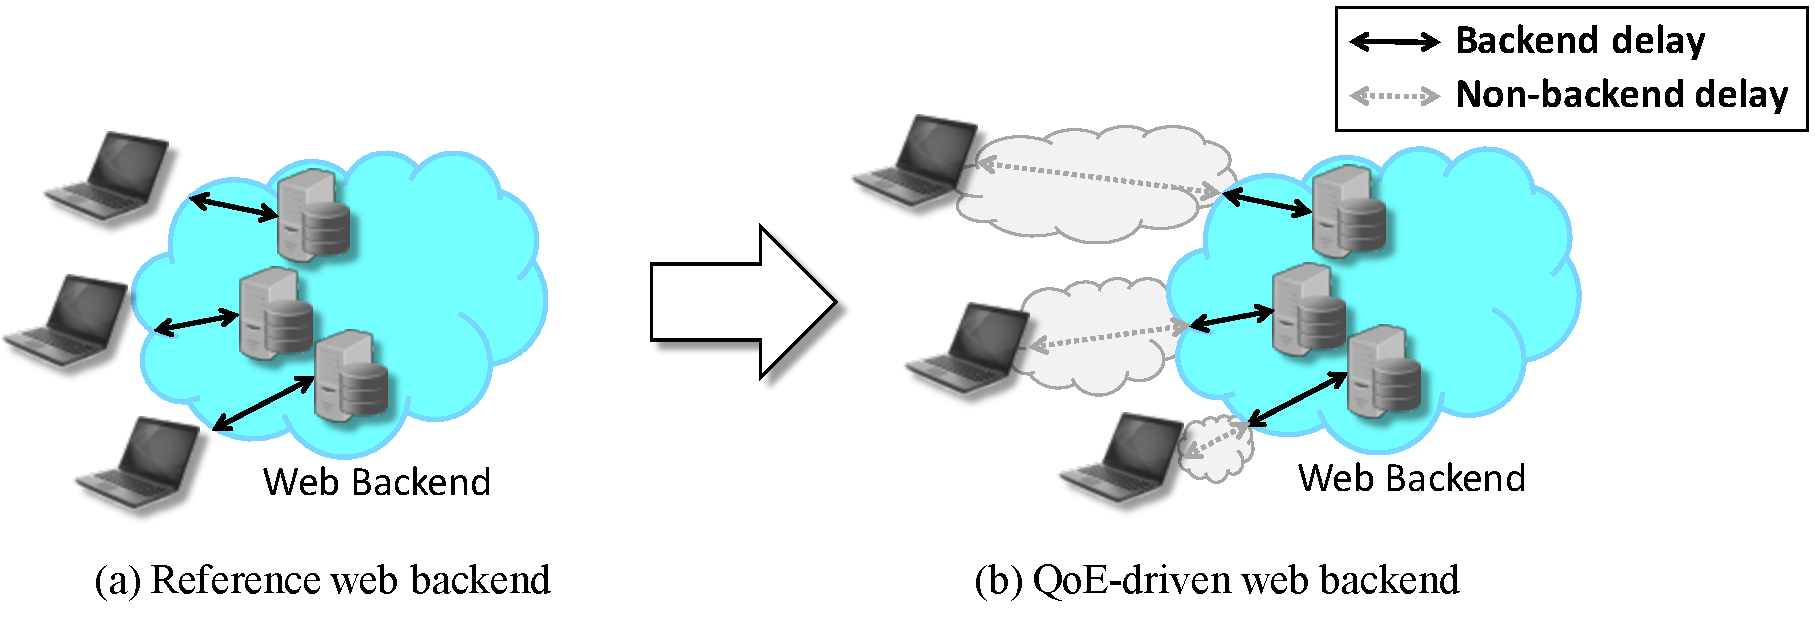
\includegraphics[width=0.75\textwidth]{figs/intro-overview.pdf}
	\vspace{-0.3cm}
	\caption{We propose to re-architect (a) today's web backend which seeks to minimize the backend delays into (b) a QoE-driven web backend which seeks to minimize the impact of backend delay on QoE.}
	\label{fig:intro-overview}
\end{figure}

%\jc{give a figure to contrast optimization of backend in-isolation vs. QoE-aware.}

%- Research goal: This project proposes that the web service backend should be aware of the QoE sensitivity. This effectively changes how one formulates the web service optimization problem.

%This proposal introduces ``QoE sensitivity'' as a new dimension for web backend QoE optimization, 
We propose to develop {\bf QoE-driven web backend} systems (Figure~\ref{fig:intro-overview}(b)). 
The key difference is that traditional backend seeks to minimize the backend delays, but a QoE-driven backend seeks to minimize the impact of backend delays on user-perceived QoE.

Despite its promise, QoE-driven backend faces two key challenges.
First, we need to estimate the real-time QoE information of each web request with sufficient accuracy when the request reaches the backend. 
Second, we need to enable QoE-driven decision-making at various subsystems of a web backend (\eg per-machine resource allocation, scheduling, replica selection).
%Through developing novel algorithms and architectural components, we show that a {\bf QoE-driven web backend} (Figure~\ref{fig:intro-overview}(b)), which is aware of and embraces the differences of QoE sensitivity across requests, can substantially {\em improve the resource/QoE tradeoffs} of web backend; \ie better QoE without using more resources, or saving resources without degrading QoE. 
% Note that being QoE sensitivity does not require expensive infrastructure changes (\eg adding hardware or changing software stack).

\mypara{Research plan}
We divide the proposed research into three tasks.
%We use the following roadmap to thoroughly examine the benefits and challenges of QoE-sensitivity-aware web service backend.

\begin{packeditemize}
\item{\bf Quantifying potential benefits (Task \#1).}
We will do measurement studies to quantify the improvements brought by the QoE-driven web backend in the wild. It will include the opportunities of QoE-driven optimizations in web backend systems, and use dataset collected from large-scale web services to understand the potential in the real-world traffic patterns.

\item{\bf Estimating per-request QoE in real time (Task \#2).}
We will develop new system components, including tracing infrastructure and QoE prediction models, to estimate the impact of backend delay on requests' QoE in real-time. We explore the possibilities of incremental deployment by reusing the existing tracing and telemetry infrastructure in today's web backend systems.

\item{\bf QoE-driven control algorithms (Task \#3).}
We will develop novel QoE-driven control policies for web backend, including resource allocation, scheduling, and replica selection. Our design goals are (1) that the policies should achieve near-optimal QoE with minimal decision-making overhead, and (2) that their implementation should be amenable to existing systems.

%\item{\bf Impact on QoE fairness (Task \#4).}
%Finally, we will explore appropriate definitions of fairness to help strike a desirable balance between QoE-driven optimization and QoE fairness. This would also help us recognize potential threads of other systems/users taking advantage of the QoE-driven policies of the backend.

\end{packeditemize}


%\jc{why these applications?}

%\jc{Common challenges! getting QoE sensitivity, fairness definition!}

\mypara{PI qualification}
The PI's expertise includes computer networking, Internet QoE, and data analytics systems.
He has published 11 peer-reviewed research papers (6 first-authored) in top-tier networking and system conferences (\ie SIGCOMM, NSDI, CoNEXT).
More importantly, the PI has a deep understanding of Internet QoE. His doctoral dissertation, titled ``Enabling Data-Driven Optimization of Quality of Experience in Internet Applications'', is among the first systematic studies to apply data-driven approach to improving Internet  QoE. The dissertation won the CMU SCS Doctoral Dissertation Award and was nominated for ACM Dissertation Award.
During his PhD and postdoctoral years, he has extensive collaborations with Microsoft Research, Conviva Inc., and Google Research. These strong connections will help the proposed research to gain insights from the industry and provide viable paths to deployment.


% \vspace{0.2cm}
% \noindent{\em Thrust \#1: How much potential benefit can we get?}

% \vspace{0.2cm}
% \noindent{\em Thrust \#2: How to re-architect web services to be QoE-aware?}

% \vspace{0.2cm}
% \noindent{\em Thrust \#3: How to propagate user-perceived QoE information?}

%- This project proposes to re-architect the web service backend by making it QoE-aware. Our roadmap has three steps.\\
%1. XXX\\
%2. YYY\\
%3. ZZZ



% \vspace{2cm}
% User-perceived quality of experience (QoE) is one of the driving forces behind the Internet ecosystem, which consists of {\em subsystems}, \eg datacenters, CDNs, cellular carriers, backbone networks, content providers, who share resources across users. 
% % End-to-end Quality of Experience (QoE) is the driving force behind today's Internet application ecosystem, which includes several subsystem
% % The Internet application ecosystem consists of many subsystems, Cloud, ISP, CDNs, etc, and 
% Thus, one fundamental question is {\em how to share resources across users in a way that optimizes their overall QoE?}
% The primary constraint is that these subsystems are {\em federated}: it is impractical to orchestrate a global optimization where they relinquish the control on how their resources are shared. 
% Instead, the conventional wisdom has been that each subsystem shares its resources among users in a way that optimizes the overall performance metrics within its limit and imposes no differentiation between users if they are ``functionally'' identical (\ie same service, business relationship, etc).

% In contrast, we are driven by a simple observation derived directly from the federated nature of the Internet ecosystem.
% In a subsystem, there is {\em a substantial heterogeneity} among its users with respect to how sensitive their QoE is to the performance of the subsystem, even if these users are functionally identical. 
% Thus, the right question to ask is {\em not} how a subsystem should optimize the overall performance among users; instead, it should minimize {\em overall impact on user-perceived QoE}, which requires treating users differently, rather than equally, depending on how much impact it has on the user's perceived QoE.

% In this proposal, we apply this idea to improving QoE of web services.

% \mypara{Research goals}

% \noindent {\bf Intellectual Merit.~~}
% This proposal applies this idea in the context of cloud services. 
% \jc{what it means to cloud services? requests are going to be treated differently, etc} 
% Specifically, this idea can be applied to many services inside a cloud. \jc{talk about more applications}
% In this project, we plan to answer three key question:

% First, how much potential benefit does this idea have?

% Second, how to design a QoE-aware cloud scheduling/resource allocation mechanism?

% Third, how to propogate QoE information from users to the cloud?

% \noindent {\bf Broader Impacts.~~}


% \noindent {\bf Keywords.~~} 



% QoE matters to everyone!

% \subsection{Missed Opportunities}
% \begin{itemize}

% \item Today's tenant: every user should be treated with the same performance goal. Implicit assumption is that the impact of a subsystem is the same on all users.

% \item However, the federated architecture means:\\
% 1. QoE can be affected by any subsystem\\
% 2. Each subsystem serves users with different QoE sensitivities.

% \item Fundamental mismatch: some users who are less sensitive to the subsystem get over-optimized, while others who are more sensitive to the subsystem get under-optimized.

% \item New approach: minimize the overall impact on QoE. 

% \end{itemize}

% \subsection{This proposal: Making Cloud QoE-Aware}
% \begin{itemize}

% \item How the cloud works today -- agnostic to QoE

% \item QoE curve

% \item Examples of how things can be done differently!

% \end{itemize}


% \subsection{Research Roadmap:}
% \begin{itemize}

% \item How much potential benefit does this idea have?

% \item How to design a QoE-aware cloud scheduling/resource allocation mechanism?

% \item How to propagate QoE information from users to the cloud?

% \end{itemize}

\end{comment}